\begin{figure}[t!]
\begin{tabular}{@{}c@{}c@{}}
\begin{subfigure}[b]{0.50\textwidth}
\begin{center}
{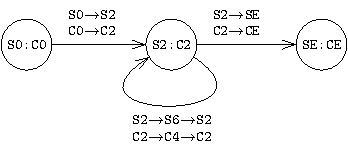
\includegraphics[scale=1.2]{chapters/figures/figStrlenArrProductCfg.pdf}}
\end{center}
\caption{\label{fig:StrlenArrProductCFG}Product-CFG for programs \cref{fig:llStrlenSpecIR,fig:llStrlenCArrIR}}
\end{subfigure}%
&
\begin{subfigure}[b]{0.50\textwidth}
\begin{center}
\begin{scriptsize}
\begin{tabular}{cl}
\toprule
{\bf PC-Pair} & \multicolumn{1}{c} {\bf Invariants} \\
\toprule
(\scpc{0}{0}) &
\Tstrut $\circled{P}\ \sv{s} \indEq{} \lifted{str}{\mem{}}{char[]}{\cv{s}}$ \\
\midrule
\multirow{2}{*}{(\scpc{2}{2})} &
\Tstrut $\circled{\tiny I1} \ \sv{s} \indEq{} \lifted{str}{\mem{}}{char[]}{\cv{s}}$ \\ &
\Tstrut $\circled{\tiny I2} \ \sv{len} = \cv{i}$ \\
\midrule
(\scpc{E}{E}) &
\Tstrut \Bstrut $\circled{E}\ \sv{ret} = \cv{ret}$ \\
\bottomrule
\end{tabular}
\end{scriptsize}
\end{center}
\caption{\label{fig:StrlenArrInvs}Invariants for product-CFG in \cref{fig:StrlenArrProductCFG}}
\end{subfigure}%
\\
\begin{subfigure}[b]{0.50\textwidth}
\begin{center}
{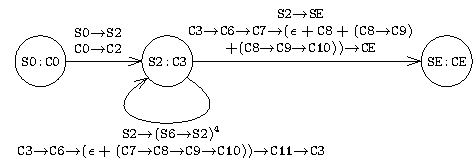
\includegraphics[scale=1.15]{chapters/figures/figStrlenClProductCfg.pdf}}
\end{center}
\caption{\label{fig:StrlenClProductCFG}Product-CFG for programs \cref{fig:llStrlenSpecIR,fig:llStrlenCClistIR}}
\end{subfigure}%
&
\begin{subfigure}[b]{0.50\textwidth}
\begin{center}
\begin{scriptsize}
\begin{tabular}{cl}
\toprule
{\bf PC-Pair} & \multicolumn{1}{c} {\bf Invariants} \\
\toprule
(\scpc{0}{0}) &
\Tstrut $\circled{P}\ \sv{s} \indEq{} \lifted{str}{\mem{}}{clnode}{\cv{cl},0}$ \\
\midrule
\multirow{2}{*}{(\scpc{2}{3})} &
\Tstrut $\circled{\tiny I1} \ \sv{s} \indEq{} \lifted{str}{\mem{}}{clnode}{\cv{cl},0}$ \\ &
\Tstrut $\circled{\tiny I2} \ \sv{len} = \cv{i}$ \\
\midrule
(\scpc{E}{E}) &
\Tstrut \Bstrut $\circled{E} \ \sv{ret} = \cv{ret}$ \\
\bottomrule
\end{tabular}
\end{scriptsize}
\end{center}
\caption{\label{fig:StrlenClInvs}Invariants for product-CFG in \cref{fig:StrlenClProductCFG}}
\end{subfigure}%
\end{tabular}
\caption{\label{fig:StrlenProductCFGsAndInvs}Product-CFGs and their node invariants representing bisimulation relations between the specification \cref{fig:llStrlenSpecIR}
and its two implementations in \cref{fig:llStrlenCArrIR,fig:llStrlenCClistIR} respectively.}
\end{figure}